\documentclass[10pt]{beamer}\usepackage[]{graphicx}\usepackage[]{color}
%% maxwidth is the original width if it is less than linewidth
%% otherwise use linewidth (to make sure the graphics do not exceed the margin)
\makeatletter
\def\maxwidth{ %
  \ifdim\Gin@nat@width>\linewidth
    \linewidth
  \else
    \Gin@nat@width
  \fi
}
\makeatother

\definecolor{fgcolor}{rgb}{0.345, 0.345, 0.345}
\newcommand{\hlnum}[1]{\textcolor[rgb]{0.686,0.059,0.569}{#1}}%
\newcommand{\hlstr}[1]{\textcolor[rgb]{0.192,0.494,0.8}{#1}}%
\newcommand{\hlcom}[1]{\textcolor[rgb]{0.678,0.584,0.686}{\textit{#1}}}%
\newcommand{\hlopt}[1]{\textcolor[rgb]{0,0,0}{#1}}%
\newcommand{\hlstd}[1]{\textcolor[rgb]{0.345,0.345,0.345}{#1}}%
\newcommand{\hlkwa}[1]{\textcolor[rgb]{0.161,0.373,0.58}{\textbf{#1}}}%
\newcommand{\hlkwb}[1]{\textcolor[rgb]{0.69,0.353,0.396}{#1}}%
\newcommand{\hlkwc}[1]{\textcolor[rgb]{0.333,0.667,0.333}{#1}}%
\newcommand{\hlkwd}[1]{\textcolor[rgb]{0.737,0.353,0.396}{\textbf{#1}}}%
\let\hlipl\hlkwb

\usepackage{framed}
\makeatletter
\newenvironment{kframe}{%
 \def\at@end@of@kframe{}%
 \ifinner\ifhmode%
  \def\at@end@of@kframe{\end{minipage}}%
  \begin{minipage}{\columnwidth}%
 \fi\fi%
 \def\FrameCommand##1{\hskip\@totalleftmargin \hskip-\fboxsep
 \colorbox{shadecolor}{##1}\hskip-\fboxsep
     % There is no \\@totalrightmargin, so:
     \hskip-\linewidth \hskip-\@totalleftmargin \hskip\columnwidth}%
 \MakeFramed {\advance\hsize-\width
   \@totalleftmargin\z@ \linewidth\hsize
   \@setminipage}}%
 {\par\unskip\endMakeFramed%
 \at@end@of@kframe}
\makeatother

\definecolor{shadecolor}{rgb}{.97, .97, .97}
\definecolor{messagecolor}{rgb}{0, 0, 0}
\definecolor{warningcolor}{rgb}{1, 0, 1}
\definecolor{errorcolor}{rgb}{1, 0, 0}
\newenvironment{knitrout}{}{} % an empty environment to be redefined in TeX

\usepackage{alltt}

\usepackage{graphicx, color}
\usepackage{alltt}
\usepackage{booktabs, calc, rotating}
\usepackage[round]{natbib}
\usepackage{pdfpages, subfigure}
\usepackage{multicol}
\usepackage{amsmath, amsbsy, amssymb, amsthm, graphicx}
\usepackage[english]{babel}
\usepackage{xkeyval} 
\usepackage{xfrac}
\usepackage{multicol}
\usepackage[normalem]{ulem}
\usepackage{multirow, fancyvrb} 
\usepackage{tikz, geometry, tkz-graph, xcolor}
\usepackage{listings}

\let\oldemptyset\emptyset
\let\emptyset\varnothing

\renewenvironment{knitrout}{\setlength{\topsep}{-.2mm}}{}

\hypersetup{colorlinks, citecolor=blue, linkcolor=., menucolor=white, filecolor=blue, anchorcolor=yellow}

\graphicspath{{figure/}}

\newcommand{\cov}{\mathrm{cov}}
\newcommand{\dif}{\mathrm{d}}
\newcommand{\dt}{\mathrm{d}t}
\newcommand{\bigbrk}{\vspace*{2in}}
\newcommand{\smallbrk}{\vspace*{.1in}}
\newcommand{\midbrk}{\vspace*{1in}}
\newcommand{\red}[1]{{\color{red}#1}}
\newcommand{\empr}[1]{{\emph{\color{red}#1}}}
\newcommand{\blue}[1]{{\color{blue}#1}}
\newcommand{\green}[1]{{\color{green}#1}}
\newcommand{\pkg}[1]{{\textbf{\texttt{#1}}}}
\newcommand{\code}[1]{{\texttt{#1}}}
\newcommand{\calc}[1]{{\fbox{\mbox{#1}}}}
\newcommand{\tp}{\hat t_p}
\newcommand{\Var}{\mathrm{Var}}
\newcommand{\SE}{\mathrm{SE}}
\newcommand{\var}{\mathrm{var}}
\newcommand{\E}{\mathrm{E}}
\newcommand{\I}{\mathrm{I}}
\newcommand{\p}{\mathrm{P}}
%\newcommand{\ll}{\textit{l}}
\newcommand{\Ss}{\widehat{S}}
\newcommand{\Skm}{\widehat{S}_{\scriptsize{KM}}}
\newcommand{\Sna}{\widehat{S}_{\scriptsize{NA}}}
\newcommand{\Hkm}{\widehat{H}_{\scriptsize{KM}}}
\newcommand{\Hna}{\widehat{H}_{\scriptsize{NA}}}
\newcommand{\V}{\mathrm{V}}
\newcommand{\R}{\texttt{R}}
\newcommand{\Cov}{\mathrm{Cov}}

\mode<presentation> {
  \usetheme{UTD}
  \usecolortheme[RGB={200,0,0}]{structure}
  \setbeamercovered{transparent}
}

\usepackage[latin1]{inputenc}
\usepackage{times}
\usepackage[T1]{fontenc}

\DeclareSymbolFont{extraup}{U}{zavm}{m}{n}
\DeclareMathSymbol{\varheart}{\mathalpha}{extraup}{86}
\DeclareMathSymbol{\vardiamond}{\mathalpha}{extraup}{87}

\newcommand*{\mybox}[1]{\framebox{#1}}

\title[STAT 6390]{STAT 6390: Analysis of Survival Data\\
  \small{Textbook coverage: Chapter 8}\\}
\author[Steven Chiou]{Steven Chiou}
\institute[UTD]{Department of Mathematical Sciences, \\ University of Texas at Dallas}
\date{}
\IfFileExists{upquote.sty}{\usepackage{upquote}}{}
\begin{document}

\begin{frame}[fragile]
  \titlepage

\end{frame}

\setbeamercolor*{item}{fg=red}
\bgroup
\usebackgroundtemplate{%
  \tikz[overlay,remember picture] \node[opacity=0.05, at=(current page.center)] {
    
\includegraphics[height=\paperheight,width=\paperwidth]{UTDbg}};}

\section{Parametric models}

\begin{frame}
  \frametitle{Parametric models}
  \begin{itemize}
  \item Methods described previously are \empr{non-parametric}; 
    no distributional assumptions were made.
  \item Non-parametric (and semi-parametric) methods have the flexibility to accommodate a wide range of applications.
  \item 
    If the assumption of a particular probability distribution for the data is valid,
    inferences based on such an assumption will be more precise. 
  \item 
    The validity of the parametric methods depends heavily on the appropriateness of the distributional assumption.
  \item 
    Parametric models are often much easier to work with. 
  \end{itemize}
\end{frame}

\begin{frame}
  \frametitle{Maximum likelihood estimation}
  \begin{itemize}
  \item 
    Suppose \empr{actual survival times} observed for $n$ individuals are $\{t_1, \ldots, t_n\}$.
  \item 
    If the probability density function of the random variable associated with theos survival times is $f(t)$, 
    the likelihood of the $n$ observations is
    \begin{equation*}
      \prod_{i = 1}^nf(t_i).
    \end{equation*}
  \item If a distributional assumption is made (e.g., $f(t) = \lambda e^{-t\lambda}$.), 
    the unkonwon parameters ($\lambda$) can be estimated by maximzing the likelihood.
  \end{itemize}
\end{frame}

\begin{frame}
  \frametitle{Maximum likelihood estimation}
  \begin{itemize}
  \item 
    Now suppose a the survival data includes (right) censored data.
  \item 
    In this case, $n$ pairs of observations are observed $(\tilde{t}_i, \Delta_i), i = 1, \ldots, n$,
    where $\tilde{T}_i$ is the observed survival time. 
  \item When $\Delta_i = 0$, $t_i$ is right-censored.
  \item The likelihood then takes the form
    \begin{equation}
      \label{eq:lik}
      L = \prod_{i = 1}^n\left[f_T(t_i)\right]^{\Delta_i}\cdot \left[S_T(t_i)\right]^{1 - \Delta_i}
      = \prod_{i = 1}^n\left[h_T(t_i)\right]^{\Delta_i}\cdot S_T(t_i).
    \end{equation}
  \item The last equation follows from the property $h(t) = f(t) / S(t)$.
  \item Note that the derivation of of $L$ does not require a distributional assumption.
  \end{itemize}
\end{frame}

\begin{frame}
  \frametitle{Maximum likelihood estimation}
  \begin{itemize}
  \item 
    A more careful derivation of the likelihood function in~\eqref{eq:lik} is to assume
    the censoring times to be random.
  \item Let $C_i$ be the random variable associated with the censoring time. 
  \item Let $\tilde{T}_i$ be the observed survival time, $\tilde{T}_i = \min(C_i, T_i)$.
  \item We will consider censored and uncensored cases separately.
  \item For the censored observation: 
    $$\p(\tilde{T}_i = t, \Delta_i = 0) = \p(C_i = t, T_i > t).$$ % = \p(C_i = t) \p(T_i > t) = f_C(t)S_T(t),$$
  \item For the uncensored observation: 
    $$\p(\tilde{T}_i = t, \Delta_i = 1) = \p(T_i = t, C_i > t).$$
  \item The likelihood is then
    \begin{equation*}
      L^* = \prod_{i = 1}^n\left[\p(T_i = t, C_i > t)\right]^{\Delta_i}\cdot\left[\p(C_i = t, T_i > t)\right]^{1 - \Delta_i}.
    \end{equation*}
  \end{itemize}
\end{frame}

\begin{frame}
  \frametitle{Maximum likelihood estimation}
  \begin{itemize}
  \item Under the assumption that $C_i$ and $T_i$ are independent, $L^*$ becomes
    \begin{equation*}
      L^* = \prod_{i = 1}^n\left[f_T(t_i)S_C(t_i)\right]^{\Delta_i}\cdot\left[f_C(t_i)S_T(t_i)\right]^{1 - \Delta_i}.
    \end{equation*}
  \item If the interest is in the parameter estimation in $f_T(\cdot)$, e.g., the $\lambda$ in the exponential assumption,
    $f_C(\cdot)$ and $S_C(\cdot)$ can be considered as constant in the maximum likelihood estimation and $L^*$ reduces to $L$.
  \item This construction shows the relevance of the assumption of independent censoring.
  \end{itemize}  
\end{frame}


\begin{frame}
  \frametitle{Exponential model}
  \begin{itemize}
  \item If a random variable, $T$, follows an exponential distribution with rate $\lambda$, then
    $$f(t) = \lambda e^{-\lambda t}, S(t) = e^{-\lambda t}, \mbox{ and } h(t) = \lambda.$$
  \item If we are willing to assumption $\{t_1, \ldots, t_n\}$ are iid samples from 
    an exponential distribution with rate $\lambda$, then the likelihood $L(\lambda)$ is 
    $$ L(\lambda) = \prod_{i = 1}^n\left[\lambda e^{-\lambda t_i} \right]^{\Delta_i} \cdot \left[ e^{-\lambda t_i}\right]^{1 - \Delta_i} = \prod_{i =1 }^n\lambda^{\Delta_i}\cdot e^{-\lambda t_i}.$$
  \item The log-likelihood is
    $$\log L(\lambda) = \ell(\lambda)= \log(\lambda)\left(\sum_{i = 1}^n\Delta_i\right) - \lambda\sum_{i = 1}^nt_i.$$
  \end{itemize}  
\end{frame}

\begin{frame}
  \frametitle{Exponential model}
  \begin{itemize}
  \item Solving for
    $$\frac{\dif \log L(\lambda)}{\dif \lambda} = \ell^\prime(\lambda) = 0 \mbox{ gives } \hat\lambda = \frac{\sum_{i = 1}^n\Delta_i}{\sum_{i = 1}^nt_i}.$$
  \item The maximum likelihood estimator (MLE), $\hat\lambda$, is the \empr{number of deaths} divides by the total survival time (\empr{number of person-years}).
  \item The MLE for the average survival time is $1 / \hat\lambda$, 
    which is the total survival time divides by the number of deaths. 
  \item With $\hat\lambda$, other quantities like the MLE for median survival times, can be derived. 
  \end{itemize}  
\end{frame}

\begin{frame}
  \frametitle{Exponential model}
  \begin{itemize}
  \item The second derivative of $\ell(\lambda)$ gives the \empr{information}.
  \item In the exponential model, we have 
    $$\ell^{\prime\prime}(\lambda) = -\frac{1}{\lambda^2}\sum_{i = 1}^n\Delta_i.$$
  \item The standard MLE theory implies
    $$\Var(\hat\lambda) \approx \frac{\hat\lambda^2}{\sum_{i = 1}^n\Delta_i}.$$
  \item The $100 (1 - \alpha)\%$ confidence interval can be constructed accordingly.
  \item The Delta method can be applied to obtain standard errors for $g(\lambda)$,
    e.g., average survival time, median survival time, etc.
  \end{itemize}  
\end{frame}

\begin{frame}
  \frametitle{Weibull model}
  \begin{itemize}
  \item The simplicity of the exponential distribution makes it attractive for some specialized applications. 
  \item A more flexibility alternative is modeling with the Weibull distribution.
  \item If $T$ follows a Weibull distribution with scale parameters $\lambda$ and shape parameter $\gamma$, 
    then
    $$ f(t) = \lambda\gamma t^{\gamma-1}e^{-\lambda t^\gamma}, S(t) = e^{-\lambda t^\gamma}, \mbox{ and } h(t) = \lambda \gamma t ^{\gamma - 1}.$$
  \item It is easy to see that when $\gamma = 1$, Weibull reduces to an exponential distribution with rate $\lambda$.
  \end{itemize}  
\end{frame}


\begin{frame}
  \frametitle{Weibull model}
  \begin{itemize}
  \item Following the similar procedure as before, the likelihood $L(\lambda, \gamma)$ is
    $$\prod_{i = 1}^n\left\{\lambda\gamma t_i^{\gamma - 1}\right\}^{\Delta_i} e^{-\lambda t_i^\gamma}.$$
  \item Let $\ell(\lambda, \gamma) = \log L(\lambda, \gamma)$, the MLE for $\lambda$ turns out to be
    $$\hat\lambda = \frac{\sum_{i = 1}^n\Delta_i}{\sum_{i = 1}^nt_i^{\hat\gamma}},$$
    but there is no close-form solution for $\hat\gamma$.
  \end{itemize}  
\end{frame}
    
\begin{frame}
  \frametitle{Weibull model}
  \begin{itemize}    
  \item The MLE $\hat\theta\equiv (\hat\lambda, \hat\gamma)$ can be obtained
    directly implementing the likelihood and optimized with \code{optim}.
  \item Numerical method like the Newton-Raphson procedure can also be used.
    % to find the value of $\hat\theta$ that maximize the likelihood function. 
  \item The basic idea of the Newton-Raphson procedure iterates 
    $$\hat\theta_{n + 1} = \hat\theta_n +
    \left(-\frac{\dif^2\ell(\hat\theta_n)}{\dif\theta^2}\right)^{-1} \cdot
    \frac{\dif\ell(\hat\theta_n)}{\dif\theta}.$$
  \item The variance-covariance matrix comes as a by-product.
  \end{itemize}  
\end{frame}

\begin{frame}
  \frametitle{Weibull model}
  \begin{itemize}
  \item Since parametric models are sensitive to the distributional assumption,
    it is important to have a diagnostic tool.
  \item A diagnostic tool for Weibull model is derived from its survival curve. 
  \item The log-log transformation of the Weibull survival function gives
    $$\log[-\log S(t)] = \log(\lambda) - \gamma\log(t).$$
  \item This suggest that if $\log[-\log S(t)]$ is plotted against $\log(t)$, 
    we would expect to see a straight line if the Weibull assumption is valid. 
  \item $S(t)$ can be replaced with $\Skm(t)$ or $\Sna(t)$.
  \end{itemize}  
\end{frame}

\begin{frame}
  \frametitle{Weibull model}
  \begin{itemize}    
  \item An alternative way is to select $\lambda$ and $\gamma$ to match the
    survival data at two specified time points.
  \item This approach is motivated by the linear relationship between $\log\left[-\log S(t)\right]$
    and $\log(t)$.
  \item Suppose we have $(t_1, s_1)$, and $(t_2, s_2)$ that are two time points on 
    a estimated survival curve (e.g., set $s_i = \Skm(t_i)$ for $i = 1, 2$).
  \item Then $\hat\lambda$ and $\hat\gamma$ can be obtained by solving the system of equation
    $$ \left\{\begin{matrix}
\log\left(-\log s_1\right) = \log(\lambda) - \gamma\log(t_1) \\ 
\log\left(-\log s_2\right) = \log(\lambda) - \gamma\log(t_2)
\end{matrix}\right.,$$
    for $\lambda$ and $\gamma$.
  \end{itemize}  
\end{frame}

\begin{frame}[fragile]
  \frametitle{Weibull model}
  \begin{itemize}
  \item The \code{Weibull2} function in the \pkg{Hmisc} package can be
    used to produce a Weibull function that matches the two points
    $(t_1, s_1)$, and $(t_2, s_2)$.
  \item Recall that $\Skm(t)$ for the \code{whas100} can be obtained with
    the \code{survfit}:

\begin{knitrout}\scriptsize
\definecolor{shadecolor}{rgb}{0.969, 0.969, 0.969}\color{fgcolor}\begin{kframe}
\begin{alltt}
\hlstd{> } \hlstd{km} \hlkwb{<-} \hlkwd{survfit}\hlstd{(}\hlkwd{Surv}\hlstd{(lenfol, fstat)} \hlopt{~} \hlnum{1}\hlstd{, whas100)}
\end{alltt}
\end{kframe}
\end{knitrout}
\item Suppose we want to find a Weibull distribution that
  matches the KM estimator at the 1st and the 6th year
  ($t = 365$ and $t = 2190$).
\begin{knitrout}\scriptsize
\definecolor{shadecolor}{rgb}{0.969, 0.969, 0.969}\color{fgcolor}\begin{kframe}
\begin{alltt}
\hlstd{> }\hlkwd{summary}\hlstd{(km,} \hlkwc{time} \hlstd{=} \hlkwd{c}\hlstd{(}\hlnum{365}\hlstd{,} \hlnum{2190}\hlstd{))}
\end{alltt}
\begin{verbatim}
Call: survfit(formula = Surv(lenfol, fstat) ~ 1, data = whas100)

 time n.risk n.event survival std.err lower 95% CI upper 95% CI
  365     80      20    0.800  0.0400        0.725        0.882
 2190     15      27    0.505  0.0537        0.410        0.622
\end{verbatim}
\end{kframe}
\end{knitrout}
\item The two points are $(365, 0.8)$ and $(2190, 0.505)$.
\end{itemize}
\end{frame}

\begin{frame}[fragile]
  \frametitle{Weibull model}
  \begin{itemize}
  \item Matching the two points with
\begin{knitrout}\scriptsize
\definecolor{shadecolor}{rgb}{0.969, 0.969, 0.969}\color{fgcolor}\begin{kframe}
\begin{alltt}
\hlstd{> }\hlstd{weiSurv} \hlkwb{<-} \hlkwd{Weibull2}\hlstd{(}\hlkwd{c}\hlstd{(}\hlnum{365}\hlstd{,} \hlnum{2190}\hlstd{),} \hlkwd{c}\hlstd{(}\hlnum{.8}\hlstd{,} \hlnum{.505}\hlstd{))}
\hlstd{> }\hlkwd{str}\hlstd{(weiSurv)}
\end{alltt}
\begin{verbatim}
function (times = NULL, alpha = 0.00560289516761242, gamma = 0.624507785991088)  
\end{verbatim}
\begin{alltt}
\hlstd{> }\hlkwd{class}\hlstd{(weiSurv)}
\end{alltt}
\begin{verbatim}
[1] "function"
\end{verbatim}
\end{kframe}
\end{knitrout}
\item \code{Weibull2} returns a function.
\item The parameters are $\lambda = 0.006$ and $\gamma = 0.625$.
\item The ``\code{alpha}'' used in \code{Weibull2} is equivalent to our $\lambda$.
\end{itemize}
\end{frame}

\begin{frame}[fragile]
  \frametitle{Weibull model}
  \begin{itemize}
  \item \code{weiSurv} returns survival probability depending on inputs.
\begin{knitrout}\scriptsize
\definecolor{shadecolor}{rgb}{0.969, 0.969, 0.969}\color{fgcolor}\begin{kframe}
\begin{alltt}
\hlstd{> }\hlkwd{weiSurv}\hlstd{(}\hlnum{365}\hlstd{)}
\end{alltt}
\begin{verbatim}
[1] 0.8
\end{verbatim}
\begin{alltt}
\hlstd{> }\hlkwd{weiSurv}\hlstd{(}\hlnum{2190}\hlstd{)}
\end{alltt}
\begin{verbatim}
[1] 0.505
\end{verbatim}
\begin{alltt}
\hlstd{> }\hlkwd{weiSurv}\hlstd{(}\hlnum{0}\hlopt{:}\hlnum{13}\hlstd{)}
\end{alltt}
\begin{verbatim}
 [1] 1.0000000 0.9944128 0.9913993 0.9889347 0.9867714 0.9848084 0.9829920
 [8] 0.9812894 0.9796788 0.9781448 0.9766759 0.9752633 0.9739001 0.9725807
\end{verbatim}
\end{kframe}
\end{knitrout}
  \end{itemize}\vspace{-.75cm}
  \begin{center}
    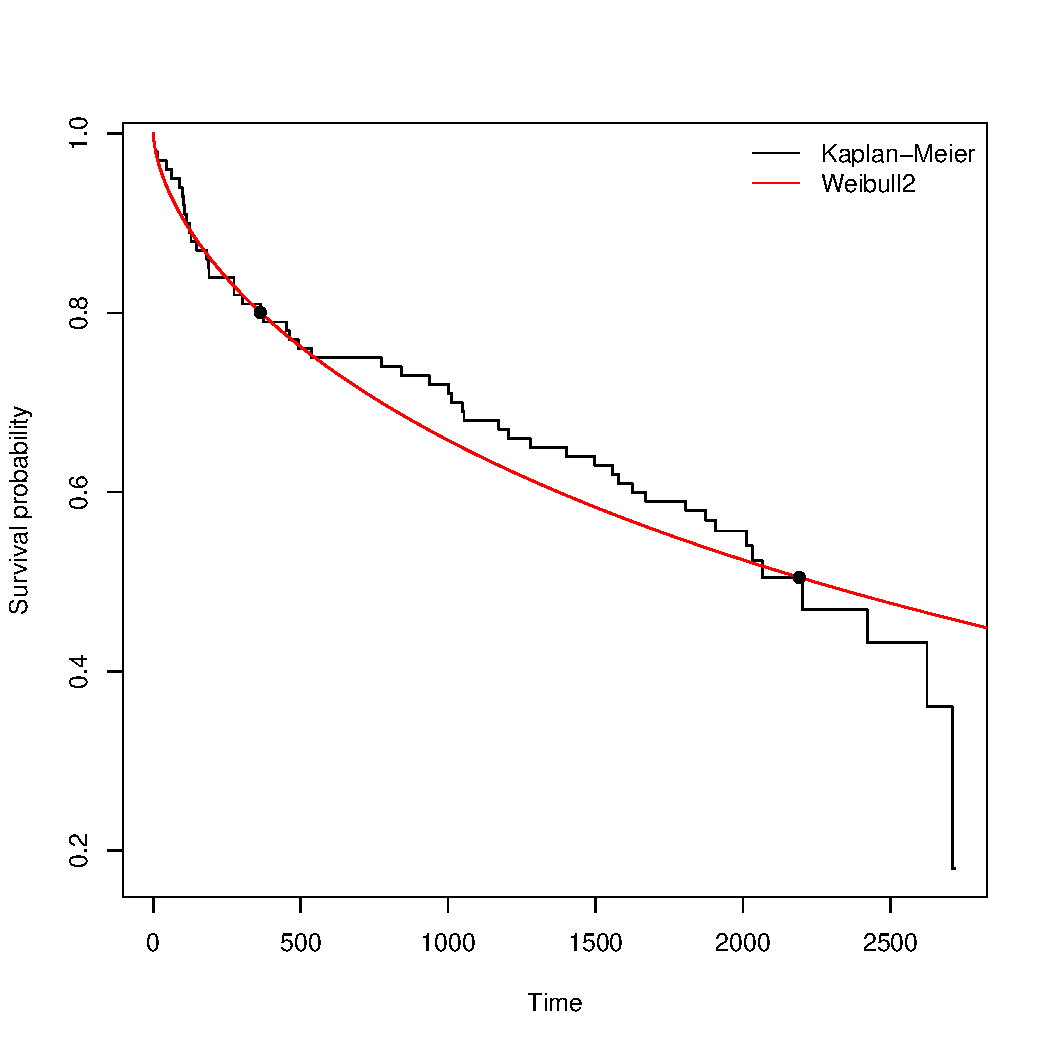
\includegraphics[scale = .32]{Weibull2}
  \end{center}
\end{frame}

\begin{frame}
  \frametitle{Exponential regression model}
  \begin{itemize}
  \item Recall that if $T$ follows an exponential distribution with rate $\lambda$,
    $T$ has the hazard function $h(t) = \lambda$.
  \item If one wants to construct a regression model under the exponential assumption,
    it is natural to model the exponential parameter $\lambda$.
  \item Suppose a covariates vector $X = (X_{1}, \ldots, X_{p})^\prime$ is available for an individual.
  \item The hazard at time $t$ for an individual can be written as
    $$\lambda(t; x) = \lambda \cdot r(X^\prime\beta),$$
    where $\beta = (\beta_1, \ldots, \beta_p)^\prime$ is the regression coefficient,
    $\lambda$ is a constant, and $r(\cdot)$ is a specified functional form.
  \end{itemize}
\end{frame}


\begin{frame}
  \frametitle{Exponential regression model}
  \begin{itemize}
  \item A few choices of $r(\cdot)$ have been proposed:
    \begin{enumerate}
    \item $r(u) = u$
    \item $r(u) = u^{-1}$
    \item $r(u) = e^u$
    \end{enumerate}
  \item The first two forms suffer from the disadvantage that $\b4ta$ must be restricted
    to guarantee $r(X^\prime\beta) > 0$ for all possible $X$.
  \item The third form is commonly considered and will be used here.
  \end{itemize}
\end{frame}

\begin{frame}
  \frametitle{Exponential regression model}
  \begin{itemize}
  \item A few choices of $r(\cdot)$ have been proposed:
    \begin{enumerate}
    \item $r(u) = u$
    \item $r(u) = u^{-1}$
    \item $r(u) = e^u$
    \end{enumerate}
  \item The first two forms suffer from the disadvantage that $\b4ta$ must be restricted
    to guarantee $r(X^\prime\beta) > 0$ for all possible $X$.
  \item The third form is commonly considered and will be used here,
    but we should keep in mind that there may be more appropriate forms in specific settings.
  \end{itemize}
\end{frame}

\begin{frame}
  \frametitle{Exponential regression model}
  \begin{itemize}
  \item Working with model with hazard function
    \begin{equation}
      \lambda(t; x) = \lambda e^{X^\prime\beta}.
      \label{eq:exp}
    \end{equation}
  \item This model specifies that log failure rate is a linear function of $X$.
  \item Setting $Y = \log(T)$, the model~\eqref{eq:exp} implies
    \begin{equation}
      \label{eq:exp-aft}
      Y = \alpha - X^\prime\beta + \epsilon,
    \end{equation}
    where $\alpha = -\log(\lambda)$ and $\epsilon$ follows an extreme value distribution.
  \item The model~\eqref{eq:exp-aft} is a log-linear model.
  \end{itemize}
\end{frame}

\begin{frame}
  \frametitle{Exponential regression model}
  \begin{itemize}
  \item The model~\eqref{eq:exp} also implies
    $$S(t;x) = \lambda t e^{X^\prime\beta},$$
    and the conditional density function of $T$ given $X$ is then
    $$f(t;x) = \lambda e^{X^\prime\beta}\cdot e^{\{- \lambda t e^{X^\prime\beta}\}}.$$
  \item Parameters can be solved by maximizing the likelihood.
  \end{itemize}
\end{frame}

\begin{frame}
  \frametitle{Weibull regression model}
  \begin{itemize}
  \item 
  \end{itemize}
\end{frame}

\end{document}




\begin{frame}[fragile]
  \frametitle{Parametric models}

\end{frame}
